\chapter{Testing With Whisker}
\label{cha:appraoch}

\section{General Approach}
\label{sec:general_appraoch}

In this work, we propose a way to perform dynamic testing on Scratch programs for Scratch 3.0.
The main goal of this approach is to be able to automatically assess student's solutions to Scratch assignments.
In order to do so, this approach makes use of an automation utility, which allows test code to
interact with running Scratch programs through Scratch's IO mechanisms.
% To enable dynamic testing for Scratch, we propose a black-bock approach with a testing utility, which allows test code to interact with a running Scratch program.
\parspace

Because Scratch's parallel scripts, as well as its lack of code separation, would make white-box testing difficult,
\mnote{Does static analysis for automated input generation make it not black-box?}
we instead chose to ignore the internals of the program and to go with a black-box approach, which only focuses on the program's input and output.
This raises the question of how to access Scratch's IO.
Since Scratch's input usually consists of mouse and keyboard input, and its output consists of visual animations and sound,
the IO is not easily accessible in a programmable way.
To overcome this challenge, we developed an automation utility called Whisker, which acts as a wrapper around Scratch.
It interacts with Scratch's virtual machine in order to automate its input and output.
Whisker offers a programmable interface for Scratch, which allows tests to simulate inputs and access information about sprites and variables.
This makes automated testing for Scratch possible.
% Selenium~\cite{selenium}, a popular tool for automated testing of web sites,
% uses a similar approach to automate web browsers.
Figure~\ref{fig:comparison_of_io_mechanisms} illustrates the difference between Scratch's IO mechanisms and Whisker's automated input and output.

\begin{figure}[htpb]
    \centering

    \begin{subfigure}[b]{\textwidth}
        \centering
        \tikzset{>=latex,
               arrow/.style={draw, -{Latex[length=1.5mm, width=1.5mm]}},
                 put/.style={draw, minimum height=1.7cm, minimum width=3.5cm, rounded corners, fill=red!20, text width=2.5cm, text centered},
                  vm/.style={draw, minimum height=3.0cm, minimum width=6.0cm, rounded corners, fill=white},
                 gui/.style={draw, minimum height=4.2cm, minimum width=7.0cm, rounded corners, fill=blue!20},
                 box/.style={draw, minimum height=4.2cm, minimum width=4.0cm, rounded corners, text width=3.5cm},
              boxtxt/.style={minimum width=4.0cm, rounded corners, text width=3.5cm}}

         \begin{tikzpicture}[scale=0.8, every node/.style={scale=0.8}]
            \begin{scope}[on background layer]
                \node[gui] at (0.0,  0.4) (gui)     {};
                \node[vm]  at (0.0,  0.0) (vm)      {};
            \end{scope}

            \node[put]     at (0.0, -0.4) (put)     {\textbf{Program under test}};
            \node[]        at (0.0,  1.0) (vmtxt)   {\textbf{Scratch Virtual Machine}};
            \node[]        at (0.0,  2.0) (guitxt)  {\large \textbf{Scratch GUI}};
            \node[box, left=of gui]       (input)   {};
            \node[box, right=of gui]      (output)  {};
            \node[boxtxt, below right] at ([yshift=-2mm] input.north west)  (inputtxt)
                {\centering {\large \textbf{Input}}\\[.5\baselineskip]Key presses, mouse movement, mouse clicks, etc.};
            \node[boxtxt, below right] at ([yshift=-2mm] output.north west) (outputtxt)
                {\centering {\large \textbf{Output}}\\[.5\baselineskip]Visual animations, audio, etc.};

            \path [arrow] (input) -- (gui);
            \path [arrow] (gui)   -- (output);
        \end{tikzpicture}
        \caption{Input and output of the Scratch GUI}
    \end{subfigure}

    \bigskip

    \begin{subfigure}[b]{\textwidth}
        \centering
        \tikzset{>=latex,
               arrow/.style={draw, -{Latex[length=1.5mm, width=1.5mm]}},
                 put/.style={draw, minimum height=1.7cm, minimum width=3.5cm, rounded corners, fill=red!20, text width=2.5cm, text centered},
                  vm/.style={draw, minimum height=3.0cm, minimum width=6.0cm, rounded corners, fill=white},
             whisker/.style={draw, minimum height=4.2cm, minimum width=7.0cm, rounded corners, fill=green!20},
                 box/.style={draw, minimum height=4.2cm, minimum width=4.0cm, rounded corners, text width=3.5cm},
              boxtxt/.style={minimum width=4.0cm, rounded corners, text width=3.5cm}}

         \begin{tikzpicture}[scale=0.8, every node/.style={scale=0.8}]
            \begin{scope}[on background layer]
                \node[whisker] at (0.0,  0.4) (whisker) {};
                \node[vm]      at (0.0,  0.0) (vm)      {};
            \end{scope}

            \node[put]         at (0.0, -0.4) (put)     {\textbf{Program under test}};
            \node[]            at (0.0,  1.0) (vmtxt)   {\textbf{Scratch Virtual Machine}};
            \node[]            at (0.0,  2.0) (guitxt)  {\large \textbf{Scratch GUI}};
            \node[box, left=of whisker]       (input)   {};
            \node[box, right=of whisker]      (output)  {};
            \node[boxtxt, below right] at ([yshift=-2mm] input.north west)  (inputtxt)
                {\centering {\large \textbf{Input}}\\[.5\baselineskip]Simulated user inputs through a programmable interface};
            \node[boxtxt, below right] at ([yshift=-2mm] output.north west) (outputtxt)
                {\centering {\large \textbf{Output}}\\[.5\baselineskip]Interface to access information about sprites and variables};

            \path [arrow] (input)   -- (whisker);
            \path [arrow] (whisker) -- (output);
        \end{tikzpicture}
        \caption{Input and output of Whisker}
    \end{subfigure}

    \caption{Comparison of IO mechanisms between the Scratch GUI and Whisker}
    \label{fig:comparison_of_io_mechanisms}
\end{figure}

\section{Testing Environment}
\label{sec:testing_environment}

Whisker is, like Scratch 3.0, implemented in JavaScript (JS).
Hence, test code is also written in JavaScript.
Whisker can theoretically be used with any JS testing framework,
but for compatibility reasons, we developed a rudimentary testing framework to go along with Whisker.
\parspace

Currently, Whisker is only available in its own web GUI, which can be seen in Figure~\ref{fig:whisker_gui}.
The web page displays Scratch's stage, a table of loaded tests, and a test report in TAP13~\cite{tap} format.
It supports batch testing more than one program with the same test suite,
but it doesn't support parallel test execution.
In the future, we plan on implementing a standalone Electron~\cite{electron} application for Whisker.
This would facilitate batch testing many programs,
and would also make it possible to test programs in parallel.
Unfortunately it is not possible to run tests in a headless environment,
because Scratch depends on a HTML canvas to render its output to.
Without a renderer, some of Scratch's blocks don't work properly.

\begin{figure}[htpb]
    \centering
    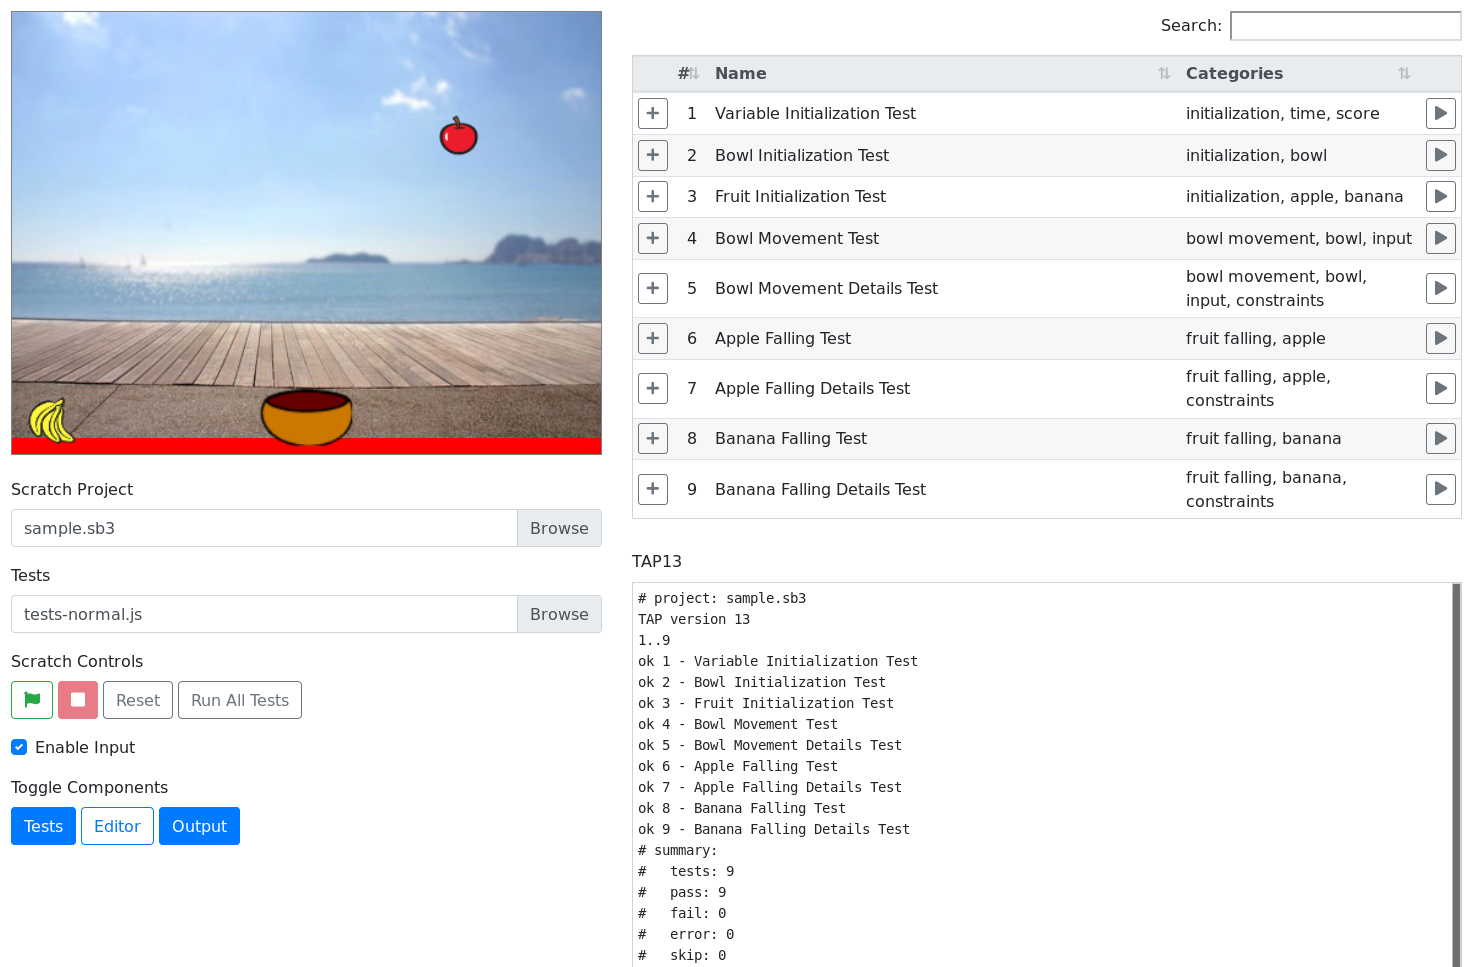
\includegraphics[width=0.85\textwidth]{whisker-gui}
    \caption{Screenshot of Whisker's web GUI}
    \label{fig:whisker_gui}
\end{figure}

\section{Public Interface}
\label{sec:public_interface}

Automating Scratch allows us to write tests for Scratch in a unit-test-like fashion.
Whisker loads the program before each test case in order to create the same initial state for every test case,
instead of going on where the last execution left off, like Scratch's GUI does it.
It also starts the program with the green flag when the test begins.
\parspace

Tests use a test driver object to automate Scratch through Whisker.
Whisker's own testing framework automatically passes the test driver object to its tests as an argument,
but tests written for other testing frameworks may have to acquire the test driver in their test code.
Whisker offers an interface to create and configure the test driver object for this purpose.
Listing~\ref{fig:examples_of_how_to_acquire_the_test_driver} shows code examples for both possibilities.
\parspace

\begin{listing}[htpb]
    \centering
    \begin{subfigure}[b]{.35\textwidth}
        \begin{minted}[autogobble, breaklines, linenos, fontsize=\scriptsize, framesep=2mm, frame=lines]{javascript}
            async function test (t) {
                ...
            }
        \end{minted}
        \vspace{-\bigskipamount}
        \caption{Getting the test driver passed as a parameter}
    \end{subfigure}
    \hspace{.05\textwidth}
    \begin{subfigure}[b]{.50\textwidth}
        \begin{minted}[autogobble, breaklines, linenos, fontsize=\scriptsize, framesep=2mm, frame=lines]{javascript}
            async function test () {
                const whisker = new WhiskerUtil(vm, project);
                whisker.prepare();
                const t = whisker.getTestDriver();
                whisker.start();
                ...
            }
        \end{minted}
        \vspace{-\bigskipamount}
        \caption{Manually acquiring the test driver through Whisker's interface}
    \end{subfigure}
    \caption{Acquiring the test driver}
    \label{fig:examples_of_how_to_acquire_the_test_driver}
\end{listing}

The following list will give an overview of Whisker's basic functions.
Because Whisker is still in early development, some of its methods may undergo changes later.
The test driver object will be denoted as $t$ in example code snippets.

\begin{itemize}
    \item \textbf{Control the program execution.}
        Tests are able to control when and for how long the program under test is run.
        In the beginning of the test, the program starts in a paused state.
        The program can then be run (resumed) for a certain time, or until a condition is met.
        Since the Scratch program execution is asynchronous, we use JavaScript's Promise API for this purpose.
        In order to simply execute the program and wait until the execution is done, the test can be declared as an \texttt{async function} and use the \texttt{await} keyword.

        The green flag can also be pressed again in order to restart the program.
        Additionally, tests can query the currently elapsed time,
        either from the start of the current program execution,
        or from the start of the test case.
        \begin{javascriptcode}
            /* Run the program for one second (1000 ms). */
            await t.runForTime(1000);
            await t.runForSteps(30);

            /* Run the program until a condition is met, with a timeout after one
             * second. The condition is given by a function that returns a boolean. */
            await t.runUntil(() => a > b, 1000);

            /* Get the total time elapsed in the current / last run. */
            t.getRunTimeElapsed();

            /* Get the total time elapsed in this test case. */
            t.getTotalTimeElapsed();

            /* Press the green flag again. */
            t.greenFlag();
        \end{javascriptcode}
    \item \textbf{Simulate Input.}
        By simulating Scratch's main input methods, tests can control the program under test.
        The goal is to simulate a user interacting with the program.
        The possible input includes mouse movement, mouse button presses, keyboard key presses, and entering answers to \texttt{ask} blocks.
        Inputs, that press (or release) a key or button, can specify a duration, after which the key is released (or pressed) again.
        Inputs can be performed immediately, or registered to be performed after a delay during the next execution.
        Inputs, that aren't performed during a run, will still trigger hats, that respond to the input.
        Tests can also query the current mouse position and if a certain key or button is pressed.
        \begin{javascriptcode}
            /* Perform a keyboard input immediately. */
            t.inputImmediate({
                device: 'keyboard',
                key: 'right arrow',
                isDown: true,
                duration: 100 // time in ms
            });

            /* Perform a mouse input one second into the next run. */
            t.addInput(1000, { device: 'mouse', x: 100, y: 200, isDown: true });

            /* Answer an ask block two seconds into the next run. */
            t.addInput(2000, { device: 'text', text: 'some answer' });

            /* Query the current state of inputs. */
            t.getMousePos(); // {x, y}
            t.isMouseDown();
            t.isKeyDown('space');
        \end{javascriptcode}
    \item \textbf{Access Scratch's output.}
        Whisker can be used to access sprites and variables of the program.
        They are accessed through sprite and variable objects, which always have the latest attributes of the sprite or variable they reference.
        Sprite objects can be obtained by their name or by their attributes.
        The provided sprite attributes include the sprite's position, rotation, size, current costume, speech bubble text, etc..
        Sprites also include the attribute values from the last execution step,
        which can be accessed through the \texttt{old} attribute of the sprite objects.
        Additionally, sprites offer some methods for detecting collisions, and other helper methods.
        \begin{javascriptcode}
            /* Various getter methods for sprites. */
                /* Get a sprite by its name. */
            const sprite = t.getSprite('Sprite1');
                /* Get sprites that match a condition. */
            const sprites = t.getSprites(sprite => sprite.x > 100);
            const clones = sprite.getClones();
            const stage = t.getStage();

            /* Various getter methods for variables. */
            const variable = stage.getVariable('my variable');
            const variables = stage.getVariables();
            const list = sprite.getList('my list');
            const lists = sprite.getLists();

            /* Accessing sprite attributes and variable values.
             * Sprites and variables always have the latest values.
             * sprite.old has the values from the last step. */
            sprite.x;
            sprite.old.x;
            variable.value;

            /* Some of the helper methods. */
            sprite.isOriginal();
            sprite.isTouchingEdge();
            sprite.isTouchingSprite(otherSprite);
        \end{javascriptcode}
    \item \textbf{Register Callbacks.}
        Tests can execute code during the program execution by registering callbacks, which get called every time the program renders a new frame.
        The can be registered to be executed before or after each frame.
        This allows tests to react to information, which the user would normally see, while the program is running.
        Callbacks can, for example, be used to track information, to perform inputs according to sprite information, or to cancel a run.
        Callbacks can be enabled and disabled.
        \begin{javascriptcode}
            /* Add a callback to be called before each step. */
            const callback = t.addCallback(() => {
                if (sprite.x > 100) {
                    t.inputImmediate({ device: 'mouse', isDown: true });
                } else if (sprite.x < 0) {
                    t.cancelRun();
                }
            });

            /* Add a callback to be called after each step (true as 2nd parameter). */
            t.addCallback(() => someList.push(sprite.x), true);

            /* Enable / disable a callback, check if a callback is active. */
            callback.disable();
            callback.enable();
            callback.isActive();
        \end{javascriptcode}
    \item \textbf{React to sprite movements and visual changes.}
        In addition to callbacks, which get called before or after each Scratch program step,
        tests can also set a function to be called whenever a sprite moves, or whenever a sprite's visuals change.
        This can be useful for detecting events, that happen during the step, but are not displayed to the user,
        which is needed for some edge cases.
        For example, let's say we test a program with two scripts:
        One of the scripts moves a sprite around.
        The other script moves the sprite back to the center of the screen whenever it touches on of the stage's edges.
        Therefore, whenever the sprite touches an edge, it is immediately moved to the center,
        even before the image is rendered.
        A normal callback will never detect the sprite touching an edge,
        but this way, detecting these collisions is possible.
        \begin{javascriptcode}
            let touchedEdge = false;

            t.onSpriteMoved(sprite => {
                touchedEdge = touchedEdge || sprite.isTouchingEdge();
            });

            t.onSpriteVisualChange(sprite => { ... });
        \end{javascriptcode}
    \item \textbf{Register constraints.}
        By registering constraints, tests can define conditions that must always hold.
        Constraints are realized through special callbacks, which perform one or more assertions.
        Whisker can be configured to fail the test on a constraint failure (the default) or to simply disable the failed constraint.
        In the second case, it is up to the test code to check which constraints failed and react accordingly.
        \begin{javascriptcode}
            /* Configure the action taken when a constraint fails. */
            t.onConstraintFailure('fail');
            t.onConstraintFailure('nothing');

            /* Check if some sprite is always visible
             * and on the right side of the screen. */
            const constraint = t.addConstraint(() => {
                t.assert.ok(sprite.visible === true, 'Sprite must always be visible.');
                t.assert.ok(sprite.x > 0, 'Sprite must always be on the right side.');
            });

            /* Enable / disable a constraint, check if a constraint is active. */
            constraint.disable();
            constraint.enable();
            constraint.isActive();
        \end{javascriptcode}
    \item \textbf{Perform randomly generated inputs.}
        Whisker provides random input generation by performing a random input from a pool of possible inputs in a constant interval during program executions.
        If a input consists of multiple events (i.e. if it has a duration) the same input cannot be chosen again while still active.
        The performed input can also be randomized itself by choosing its values randomly from a configured interval.
        Tests can either provide the pool or inputs themselves or let Whisker determine what inputs the program reacts to through static analysis.
        The time interval in which random inputs are performed can also be configured.
        \begin{javascriptcode}
            /* Set the interval, how often random inputs should be performed. */
            t.setRandomInputInterval(150);

            /* Register random inputs for the pool manually. */
            t.registerRandomInputs([
                  { device: 'keyboard', key: 'left arrow', duration: [50, 100] },
                  { device: 'keyboard', key: 'right arrow', duration: [50, 100] },
                  { device: 'mouse', x: [-100, 100], y: [-100, 100] }
            ]);

            /* Let Whisker detect inputs for the pool. */
            t.detectRandomInputs({ duration: [50, 100] });
        \end{javascriptcode}
\end{itemize}
\parspace

% \noindent Despite being possible in theory, Whisker does not provide the means to execute single scripts or blocks of the program directly.
% \mnote{TODO: really write about grading here?}
% It only allows executing the program as a whole.
% This has two reasons.
% Since the main goal for this testing approach is automated grading, one test suite is possibly executed on a large number of different implementations.
% Therefore, we don't want to concern ourselves with the internals of the program, since they may change from program to program.
% Secondly, executing single scripts could also lead to unexpected behaviour in the program, because scripts in typical Scratch programs often depend on other scripts, which run in parallel.
% This is mainly due to the game-like nature of usual Scratch programs.
% They often feature multiple sprites running loops in order to be interactive.

\section{Challenges of this Approach}
\label{sec:appraoch_challenges}

% \begin{itemize}
%     \item This approach allows to test programs with most of Scratch's functionality.
%         Apart from sounds and extensions, anything, which Scratch has to offer, can be tested with this approach.
%         In contrast, ITCH's previous testing approach limited Scratch programs to textual IO.
%     \item Tests are easily understood, because they control the program like a normal person would.
%     \mnote{Can't state this without proof $\rightarrow$ "we believe" or similar}
%         This is important, because students, whose programs are supposed to be tested later,
%         could be allowed to run tests on their programs themselves during development.
%         This way, students could easily receive valuable feedback about the correctness of their implementations.
%         Therefore, it is beneficial to use tests, whose actions and purposes are easily understood by students.
% \end{itemize}

This section highlights various challenges that one can face when using this approach.%
\parspace

\textbf{General testing challenges.}
Firstly, automated dynamic testing in general introduces some challenges.
For one thing, programs have to be well specified, since testing relies on the program's specification.
Therefore, if the specification is too vague, testing can become difficult.
Tests for imprecise specifications potentially need to consider more possible cases of how the program could behave.
Likewise, conflicting interpretations of the specification between the test and the program may result in false negative test outcomes.
Also, since we only test the program as a whole, testing a single part of the program can be difficult.
If some feature of the program under test depends on another feature being implemented correctly,
but the latter does not work, the first feature can not be tested properly.
\parspace

\textbf{Addressing sprites and variables.}
In order to access information about sprites and variables, they need to be addressed in some way.
Sprites can be addressed by their name or by any of their attributes, for example by their position.
Nevertheless, if a sprite, that is needed for the test, can not be found, the test can not work properly.
This can be a problem if a Scratch program deviates from the specification.
For example, if students are given a template with sprite names already in place,
some students could rename the sprites form the template, causing tests to fail.
However, errors like this can easily be detected through test reports.
% Probably the easiest way to handle this is to give students a Scratch project with the sprites and variables already in place
% as a template so the sprites and variables have the same name in each student solution.
\parspace

\textbf{Missing initialization.}
Another challenge are programs with missing initialization which are saved in a bad state.
When the green flag is pressed, the Scratch GUI simply picks up where the last execution left off.
Therefore, students might not initialize their program properly,
which can cause it to sometimes behave incorrectly when the green flag is pressed.
A program with missing initialization may be saved in a bad state,
meaning the program will behave incorrectly the next time it is started.
Since we restore the same state in the beginning of each test case,
such a program will always behave incorrectly during the tests although the implementation might be mostly correct.
\parspace

\textbf{Time-displaced events.}
Programs may have events that are supposed to trigger certain actions.
For example, a sprite touching another sprite may cause a variable to be incremented.
But the exact timing for the triggered action is often unknown, because the event is detected through a loop.
Therefore, tests have to check if the action happens in a time interval after the event occurred.
This may be done by tracking timestamps of the event and the action, and comparing these timestamps,
but this can be expensive to do.
\parspace

\chapter{Using Constraints For Flexible Test Inputs}
\label{cha:using_constraints_for_flexible_test_inputs}

This section will describe why separating control of the program under test from the test code can be beneficial,
and how this can be achieved by defining constraints, that are checked in the background.

\section{Input-Independent / Constraint-only Tests}
\label{sec:input_independent_constraint_only_tests}

\mnote{TODO: ''constraint-only''}
Usually, tests will provide the program under test with inputs and check the resulting outputs.
However, in many cases, a different approach is possible as well.
Tests may use other sources of input and simply observe if the program's output is correct for the input provided by the source.
QuickCheck~\cite{quickcheck} by Claessen et al., for example, uses this principle, to test the correctness of Haskell programs.
In order to do so, tests define conditions, which the program must comply with.
QuickCheck then automatically generates input for the program and checks if the defined conditions hold.
\parspace

Scratch programs can often be tested in a similar way.
But in order to be able to do this, tests have to be made independent of the simulated input on the program.
This will not just enable us to test with generated input, but with other input sources as well.
For example, the program could be manually controlled by a person, or input could be recorded and played back.
Whisker also offers its own implementation of automated input generation.
% Whisker also offers its own method of automated input generation by randomizing a set of inputs,
% which are either provided by the test itself, or deduced by analyzing the program code (see section~\ref{sec:automated_input_generation} for more information on this).
\parspace

% Scratch tests can often be made independent of inputs, and Whisker provides the means to do this.
Using constraints allows us to define conditions, which the program must hold.
Constraints check the program's compliance to the conditions by continually performing assertions throughout the program execution.
Since this is done entirely in the background while the program under test is running, we can define constraints and just let the program run for some time.
This way, it does not matter in what state the program is during its execution, or what inputs it is receiving.
If a condition does not hold, the respective constraint fails.

\section{Testing Procedure}
\label{sec:constraint_testing_procedure}

Figure~\ref{fig:input_independent_testing_procedure} shows a testing procedure, which uses the aforementioned approach to test independently of the simulated input.
We will go through each step of the procedure with the aid of an example.
Consider a program with a single sprite, which is supposed to move to the right when, and only when, the right arrow key is pressed.
We want to write a test to check if the sprite's movement works correctly.
For the sake of simplicity we are going to ignore the case of the sprite not being able to move right when touching the right edge of the screen.

\begin{figure}[htpb]
    \centering
    \tikzset{>=latex,
           arrow/.style={draw, -{Latex[length=1.5mm, width=1.5mm]}},
             box/.style={draw, text width=4.3cm, minimum height=0.7cm, text centered, rounded corners},
             num/.style={draw, circle, inner sep=0.6mm, text centered},
               h/.style={fill=blue!10}}

    \begin{tikzpicture}[scale=0.9, every node/.style={scale=0.9}]
        \node[box]    at (0.2, 5.75) (initialize)  {(Give the program some time to Initialize)};
        \node[box, h] at (0.2, 4.25) (tracking)    {Setup information tracking};
        \node[box, h] at (0.2, 3.0)  (constraints) {Register constraints};
        \node[box]    at (0.2, 2.0)  (inputs)      {(Simulate Inputs)};
        \node[box]    at (0.2, 1.0)  (run)         {Run the program};
        \node[box, h] at (0.2, 0.0)  (verify)      {Verify tested situation};

        \node[num] at (-2.6, 5.75) (one)   {1};
        \node[num] at (-2.6, 4.25) (two)   {2};
        \node[num] at (-2.6, 3.0)  (three) {3};
        \node[num] at (-2.6, 2.0)  (four)  {4};
        \node[num] at (-2.6, 1.0)  (five)  {5};
        \node[num] at (-2.6, 0.0)  (six)   {6};

        \draw[arrow]
               (0.2,  6.6)
            -- (initialize)
            -- (tracking)
            -- (constraints)
            -- (inputs)
            -- (run)
            -- (verify)
            -- (0.2, -0.8);
    \end{tikzpicture}

    \caption{Input-independent / constraint-only testing procedure}
    \label{fig:input_independent_testing_procedure}
\end{figure}

\begin{enumerate}
    \item[(1)] \textbf{Give the program some time to initialize.}
        Before setting up any tracking or registering constraints we may need to run the program for a short time.
        Otherwise the initialization of the program might be tracked, which will lead to wrong test results.
        \begin{javascriptcode}
            t.runForTime(100);
        \end{javascriptcode}
    \item[(2)] \textbf{Setup information tracking.}
        Since the sprite might not move right in the same step the right arrow key is pressed,
        we want to accept slightly delayed movement in the test.
        For this purpose, we track the timestamps when the key starts being pressed,
        when the key was last pressed, and when the sprite last moved.
        We also record if the right arrow key was pressed (and released) at all,
        so we can verify it being pressed (and released) in the end of the test.
        \begin{javascriptcode}
            /* When the last right arrow key press started. */
            let startPressedTime = undefined;
            /* When the right arrow key was last recorded being pressed. */
            let pressedTime = undefined;
            /* When the sprite was last recorded moving right. */
            let movedRightTime = undefined;
            /* If the right arrow key was pressed in the previous step. */
            let previouslyPressed = t.isKeyDown('right arrow');
            /* If the right arrow key was pressed (and released) at all. */
            let pressed = false, released = false;

            const trackRightKeyCb = t.addCallback(() => {
                const currentTime = t.getTotalTimeElapsed();
                if (t.isKeyDown('right arrow')) {
                    pressedTime = currentTime;
                    if (!previouslyPressed) {
                        startPressedTime = currentTime;
                    }
                    previouslyPressed = true;
                    pressed = true;
                } else {
                    previouslyPressed = false;
                    released = true;
                }
            });

            const trackSpriteMoveCb = t.addCallback(() => {
                if (sprite.x > sprite.old.x) {
                    movedRightTime = t.getTotalTimeElapsed();
                }
            });
        \end{javascriptcode}
    \item[(3)] \textbf{Register constraints.}
        Since we tracked when the time when the key was pressed and when the sprite last moved,
        we add a constraint that simply compares the timestamps to determine if the sprite moved at the correct times.
        We chose to allow a delay of $100~\text{ms}$ for the sprite to react to the right arrow key being pressed or being released.
        We also register a second constraint, that checks that the sprite only ever stays still or moves to the right,
        but never moves in any other direction.
        \begin{javascriptcode}
            const moveTimingsConstraint = t.addConstraint(() => {
                const currentTime = t.getTotalTimeElapsed();
                if (currentTime > startPressedTime + 100) {
                    t.assert.ok(Math.abs(movedRightTime - pressedTime) <= 100,
                        'Sprite must move right when, and only when, the right arrow key is pressed.');
                }
            });

            const moveDirectionConstraint = t.addConstraint(() => {
                t.assert.ok(sprite.x >= sprite.old.x,
                    'Sprite must only stand still or move right');
                t.assert.ok(sprite.y == sprite.old.y,
                    'Sprite must not move vertically.');
            });
        \end{javascriptcode}
    \item[(4,5)] \textbf{Simulate Inputs, Run the program.}
        Now we may register inputs if we want to, and then we can run the program.
        How we simulate inputs, or if we perform inputs manually, does not matter for the test, of course.
        \begin{javascriptcode}
            t.setRandomInputInterval(250);
            t.detectRandomInputs();

            await t.runForTime(1000);
        \end{javascriptcode}
    \item[(6)] \textbf{Verify tested situation.}
        If our source of input does not guarantee that the right arrow key gets pressed at all, we risk the chance of a false positive test result,
        since the test never expects the sprite to move right.
        A similar problem occurs when the key is always pressed.
        Therefore, we want to skip the test if either the right arrow key was never pressed,
        or was pressed the whole time.
        \begin{javascriptcode}
            t.assume.ok(pressed, 'Right arrow key must be pressed.');
            t.assume.ok(released, 'Right arrow key must be released.');
        \end{javascriptcode}
\end{enumerate}
\parspace

Figure~\ref{fig:normal_input_independent_test_comparison} shows the resulting test code for the example
and compares it to a similar test, which simulates inputs deliberately to check the sprite's movement.
We can easily see, that this approach takes quite a bit more code than the more normal approach.
But at the same time, the input-independent testing procedure is able to scale better than the other testing procedure.
Once enough tracking is set up, writing constraints becomes easy and requires little code.
At the same time, because the constraints are isolated from the program execution itself,
many constraints can possibly be combined into a single test.
For this purpose, Whisker offers an option to disable failed constraints instead of failing the entire test.
In this case, tests can simply check which constraints failed, and let Whisker generate a test report from them.

\begin{listing}[htpb]
    \centering
    \begin{subfigure}[b]{.40\textwidth}
        \centering
        \begin{minted}[autogobble, breaklines, linenos, fontsize=\tiny, framesep=2mm, frame=lines]{javascript}
            const sprite = t.getSprite('Sprite1');

            /* Give the program some time to initialize. */
            await t.runForTime(100);

            let oldX = sprite.x;

            /* Check that the sprite never moves into an other
             * direction that right. */
            t.addConstraint(() => {
                t.assert.ok(sprite.x >= sprite.old.x,
                    'Sprite must only stand still or move right');
            });

            /* Run without inputs and check that the sprite
             * doesn't move. */

            await t.runForTime(1000);

            t.assert.ok(oldX === sprite.x,
                'Sprite must not move right when no key is pressed.');

            /* Run with the right arrow key being pressed and
             * check that the sprite moves to the right. */

            t.inputImmediate({
                device: 'keyboard',
                key: 'right arrow',
                isDown: true
            });

            await t.runForTime(1000);

            t.assert.ok(oldX < sprite.x,
                'Sprite must move right when right arrow key is pressed.');
        \end{minted}
        \vspace{-\bigskipamount}
        \caption{Normal test}
    \end{subfigure}
    \hspace{.08\textwidth}
    \begin{subfigure}[b]{.50\textwidth}
        \centering
        \begin{minted}[autogobble, breaklines, linenos, fontsize=\tiny, framesep=2mm, frame=lines]{javascript}
            let sprite = t.getSprite('Sprite1');

            /* (1) Give the program some time to initialize. */
            await t.runForTime(100);

            /* When the last right arrow key press started. */
            let startPressedTime = undefined;
            /* When the right arrow key was last recorded being pressed. */
            let pressedTime = undefined;
            /* When the sprite was last recorded moving right. */
            let movedRightTime = undefined;
            /* If the right arrow key was pressed in the previous step. */
            let previouslyPressed = t.isKeyDown('right arrow');
            /* If the right arrow key was pressed (and released) at all. */
            let pressed = false, released = false;

            /* (2) Track when the right arrow key is being pressed,
             * and when the sprite is moving to the right. */

            const trackRightKeyCb = t.addCallback(() => {
                const currentTime = t.getTotalTimeElapsed();
                if (t.isKeyDown('right arrow')) {
                    pressedTime = currentTime;
                    if (!previouslyPressed) {
                        startPressedTime = currentTime;
                    }
                    previouslyPressed = true;
                    pressed = true;
                } else {
                    previouslyPressed = false;
                    released = true;
                }
            });

            const trackSpriteMoveCb = t.addCallback(() => {
                if (sprite.x > sprite.old.x) {
                    movedRightTime = t.getTotalTimeElapsed();
                }
            });

            /* (3) Check if the sprite only moves when the right arrow
             * key was pressed, and if it doesn't move when the key was
             * not pressed. */

            const moveTimingsConstraint = t.addConstraint(() => {
                const currentTime = t.getTotalTimeElapsed();
                if (currentTime > startPressedTime + 100) {
                    t.assert.ok(Math.abs(movedRightTime - pressedTime) <= 100,
                        'Sprite must move right when, and only when, the right arrow key is pressed.');
                }
            }));

            const moveDirectionConstraint = t.addConstraint(() => {
                t.assert.ok(sprite.x >= sprite.old.x,
                    'Sprite must only stand still or move right');
                t.assert.ok(sprite.y == sprite.old.y,
                    'Sprite must not move vertically.');
            }));

            /* (4) Some code, which registers inputs. Or nothing if
             * inputs are done manually. For example, generated input: */
            t.setRandomInputInterval(250);
            t.detectRandomInputs();

            /* (5) Run the program. */
            await t.runForTime(5000);

            /* (6) Check if the right arrow key was pressed at all,
             * and if it was ever released. */
            t.assume.ok(pressed, 'Right arrow key must be pressed.');
            t.assume.ok(released, 'Right arrow key must be released.');
        \end{minted}
        \vspace{-\bigskipamount}
        \caption{Input-independent test}
        \label{fig:normal_input_independent_test_comparison_constraint}
    \end{subfigure}
    \caption{Comparison of normal tests and an input-independent tests}
    \label{fig:normal_input_independent_test_comparison}
\end{listing}

\section{Resetting the Program During a Test}
\label{sec:resetting_the_program_during_a_test}

When testing with randomly generated input, programs often need to be reset multiple times inside of one test execution,
because the test could get stuck in some state of the program.
\parspace

To reset a Scratch program, we may simply press the green flag button again,
but we also need to consider the tracked information as well as the registered callbacks and constraints when resetting the program under test.
Any per-run information we tracked has to be cleared, and callbacks as well as constraints have to disabled before resetting the program.
After resetting the program, callbacks and constraints have to be enabled again.
Also, if the test configured Whisker not to fail the test when a constraint fails, then the test needs to check which constraints failed before disabling them
and then only enable constraints which were active before.
Figure~\ref{fig:resetting_the_program_under_test_procedure} shows a procedure that may be used to reset the program under test.
This procedure replaces step $5$ (Run the program) in the input-independent testing procedure (see Figure~\ref{fig:input_independent_testing_procedure}).
Additionally the code example in Listing~\ref{fig:resetting_the_program_under_test_example}
implements this procedure for the example from the previous section.
\parspace

Sometimes, information may need to be tracked across resets in order to determine what events occurred in the program during the whole test execution.
This information may be needed to rule out constraints, whose situation never occurred, after the test execution.
An example for this are the variables \texttt{pressed} and \texttt{released} in Listing~\ref{fig:normal_input_independent_test_comparison_constraint}.
\parspace


\begin{figure}[htpb]
    \centering
    \begin{subfigure}[m]{.3\textwidth}
        \centering
        \tikzset{>=latex,
               arrow/.style={draw, -{Latex[length=1.5mm, width=1.5mm]}},
                 box/.style={draw, text width=4.3cm, minimum height=0.7cm, text centered, rounded corners},
                 num/.style={draw, circle, inner sep=0.6mm, text centered},
                   h/.style={fill=blue!10}}

        \begin{tikzpicture}[scale=0.9, every node/.style={scale=0.9}]
            \node[box, h] at (0.2,  6.75) (suspendcb)  {Suspend Information Tracking};
            \node[box, h] at (0.2,  5.50) (suspendcn)  {Suspend Constraints};
            \node[box, h] at (0.2,  4.25) (resetinfo)  {Reset per-run information};
            \node[box]    at (0.2,  2.25) (greenflag)  {Press the green flag (and give the program some time to Initialize)};
            \node[box]    at (0.2,  0.75) (spriteref)  {Get new sprites};
            \node[box, h] at (0.2, -0.75) (activatecb) {Activate Information Tracking};
            \node[box, h] at (0.2, -2.00) (activatecn) {Activate Constraints};
            \node[box]    at (0.2, -3.00) (run)        {Run the program};


            \node[num] at (-2.6,  6.75) (one)   {1};
            \node[num] at (-2.6,  5.50) (two)   {2};
            \node[num] at (-2.6,  4.25) (three) {3};
            \node[num] at (-2.6,  2.25) (four)  {4};
            \node[num] at (-2.6,  0.75) (five)  {5};
            \node[num] at (-2.6, -0.75) (six)   {6};
            \node[num] at (-2.6, -2.00) (seven) {7};
            \node[num] at (-2.6, -3.00) (eight) {8};

            \draw[arrow]
                   ( 0.2,  7.6)
                -- (suspendcb)
                -- (suspendcn)
                -- (resetinfo)
                -- (greenflag)
                -- (spriteref)
                -- (activatecb)
                -- (activatecn)
                -- (run)
                -- ( 0.2, -3.8);

            % \draw[-, rounded corners]
            %        ( 0.2, -2.8)
            %     -- (-3.4, -2.8)
            %     -- (-3.4,  7.7)
            %     -- ( 0.2,  7.7);
        \end{tikzpicture}
        \caption{Procedure for resetting the program under test}
        \label{fig:resetting_the_program_under_test_procedure}
    \end{subfigure}%
    \hspace{.13\textwidth}%
    \begin{subfigure}[m]{.55\textwidth}
        \centering
        \begin{minted}[autogobble, breaklines, linenos, fontsize=\scriptsize, framesep=2mm, frame=lines]{javascript}
            for (let i = 0; i < 5; i++) {
                const constraints = [moveTimingsConstraint,
                    moveDirectionConstraint];

                /* (1) Suspend information tracking. */
                trackRightKeyCb.disable();
                trackSpriteMoveCb.disable();

                /* (2) Suspend constraints.
                 * Get a list active constraints first.
                 * (Constraints that did not fail) */
                const ac = constraints.filter(c => c.isActive());
                for (const constraint of ac) {
                    constraint.disable();
                }

                /* (3) Reset per-run information
                   (keep values of 'pressed' and 'released'). */
                startPressedTime = undefined;
                pressedTime = undefined;
                movedRightTime = undefined;
                previouslyPressed = t.isKeyDown('right arrow');

                /* (4) Press the green flag and give the program
                   some time to Initialize. */
                t.greenFlag();
                await t.runForTime(100);

                /* (5) Get new sprites. */
                let sprite = t.getSprite('Sprite1');

                /* (6) Activate information tracking. */
                trackRightKeyCb.enable();
                trackSpriteMoveCb.enable();

                /* (7) Activate constraints. */
                for (const constraint of ac) {
                    constraint.enable();
                }

                /* (8) Run the program. */
                await t.runForTime(2000);
            }
        \end{minted}
        \vspace{-\bigskipamount}
        \caption{Example code for resetting the program under test (extends Listing~\ref{fig:normal_input_independent_test_comparison_constraint})}
        \label{fig:resetting_the_program_under_test_example}
    \end{subfigure}

    \caption{Resetting the program under test}
    \label{fig:resetting_the_program_under_test}
\end{figure}


% Register Callbacks for Information Tracking (per run for constraints and across runs to rule out constraints in the end)
% Register Constraints
%
% repeat:
%     Suspend Information Tracking Callbacks
%     Suspend Constraints
%
%     Reset Per Run Information
%
%     Press Green Flag
%     Run the Program For Short Time to Initialize It
%
%     Activate Information Tracking Callbacks
%     Activate Constraints
%
%     Run the Program
%
% Check Across-Run Information to Disable Constraints, whose situation to check did not occur
% Generate test report


% \begin{figure}[htpb]
%     \centering
%     \begin{subfigure}[b]{.45\textwidth}
%         \centering
%         \tikzset{>=latex,
%                  box/.style={draw, text width=4.3cm, minimum height=0.7cm, text centered, rounded corners},
%                  num/.style={draw, circle, inner sep=0.6mm, text centered},
%                    h/.style={fill=blue!10}}
%
%         \begin{tikzpicture}
%             \node[box] at ( 0.2,  3.0) (run)        {Run the program};
%             \node[box] at ( 0.2,  2.0) (inputs)     {Simulate inputs};
%             \node[box] at ( 0.2,  1.0) (checks)     {Perform checks};
%
%             \node[num] at (-2.6,  3.0) (one)   {1};
%             \node[num] at (-2.6,  2.0) (two)   {2};
%             \node[num] at (-2.6,  1.0) (three) {3};
%
%             \draw[->]
%                    ( 0.2,  4.8)
%                 -- (run)
%                 -- (inputs)
%                 -- (checks)
%                 -- ( 0.2, -1.0);
%
%             \draw[shorten >= 2pt, rounded corners, dashed, ->]
%                    ( 0.2,  0.0)
%                 -- (-3.4,  0.0)
%                 -- (-3.4,  4.0)
%                 -- ( 0.2,  4.0);
%         \end{tikzpicture}
%
%         \caption{Normal Test Procedure}
%         \label{fig:normal_test_procedure}
%     \end{subfigure}
%     \begin{subfigure}[b]{.45\textwidth}
%         \centering
%         \tikzset{>=latex,
%                  box/.style={draw, text width=4.3cm, minimum height=0.7cm, text centered, rounded corners},
%                  num/.style={draw, circle, inner sep=0.6mm, text centered},
%                    h/.style={fill=blue!10}}
%
%         \begin{tikzpicture}
%             \node[box] at ( 0.2,  4.25) (tracking)    {Setup tracking of information};
%             \node[box] at ( 0.2,  3.0)  (constraints) {Register constraints};
%             \node[box] at ( 0.2,  2.0)  (run)         {Run the program};
%             \node[box] at ( 0.2,  1.0)  (inputs)      {(Simulate Inputs)};
%             \node[box] at ( 0.2,  0.0)  (filter)      {Filter constraints};
%
%             \node[num] at (-2.6,  4.25) (one)   {1};
%             \node[num] at (-2.6,  3.0)  (two)   {2};
%             \node[num] at (-2.6,  2.0)  (three) {3};
%             \node[num] at (-2.6,  1.0)  (four)  {4};
%             \node[num] at (-2.6,  0.0)  (five)  {5};
%
%             \draw[->]
%                    (tracking)
%                 -- (constraints)
%                 -- (run)
%                 -- (inputs)
%                 -- (filter)
%                 -- ( 0.2, -1.0);
%         \end{tikzpicture}
%
%         \caption{Constraint-only Test Procedure}
%         \label{fig:constraint_only_test_procedure}
%     \end{subfigure}
%     \caption{Comparison of the procedure of normal tests and constraint-only tests}
%     \label{fig:comparison_of_the_procedure_of_normal_tests_and_constraint_only_tests}
% \end{figure}
